\subsubsection{Implementazione dell'AST}
L'output della fase di parsing è un oggetto di tipo \texttt{FileRepresentation}. Esso 
è sostanzialmente la radice dell'AST relativo ad un singolo file sorgente, ed è 
composto da una collezione di radici di sotto-alberi corrispondenti alle definizioni contenute 
nel file. \\

\vspace{0.5cm}
\begin{lstlisting}[language=C++, frame=single]
struct FileRepresentation {

    struct Metadata {
        string filename;
        string packagename;
        vector<string> imports;
    };

    Metadata file_metadata;
    vector<TypeDefinition> type_defs;
    vector<FunctionDefinition> func_defs;
};
\end{lstlisting}
\vspace{0.5cm}

La classe \texttt{TypeDefinition} rappresenta una definizione di tipo, ed è super-tipo
di tutti i nodi dell'AST che rappresentano definizioni di tipo. \\

\begin{figure}[H]
    \centering
        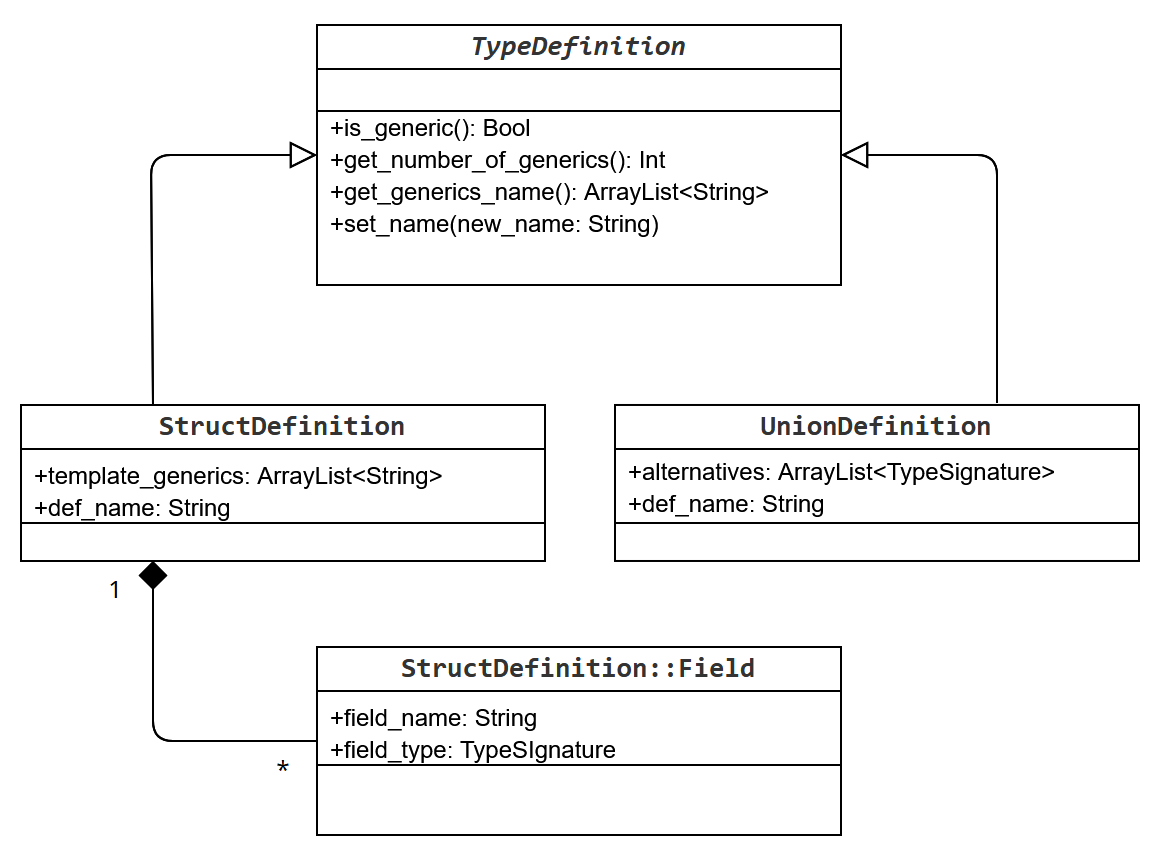
\includegraphics[width=0.7\textwidth]{../../Assets/TypeDefAST.png}
    \caption{
        \centering
        UML class diagram dei nodi dell'AST che rappresentano le definizioni di tipo
    }
\end{figure}

\newpage

Di seguito segue l'UML class diagram relativo alle classi che modellano 
le espressioni in forma di AST. Si tenga presente che anche la repository
basata su ANTLR utilizza la medesima rappresentazione, e si utilizza il visitor 
autogenerato da ANTLR per navigare la rappresentazione di ANTLR e tradurla opportunamente.

\begin{figure}[H]
    \centering
        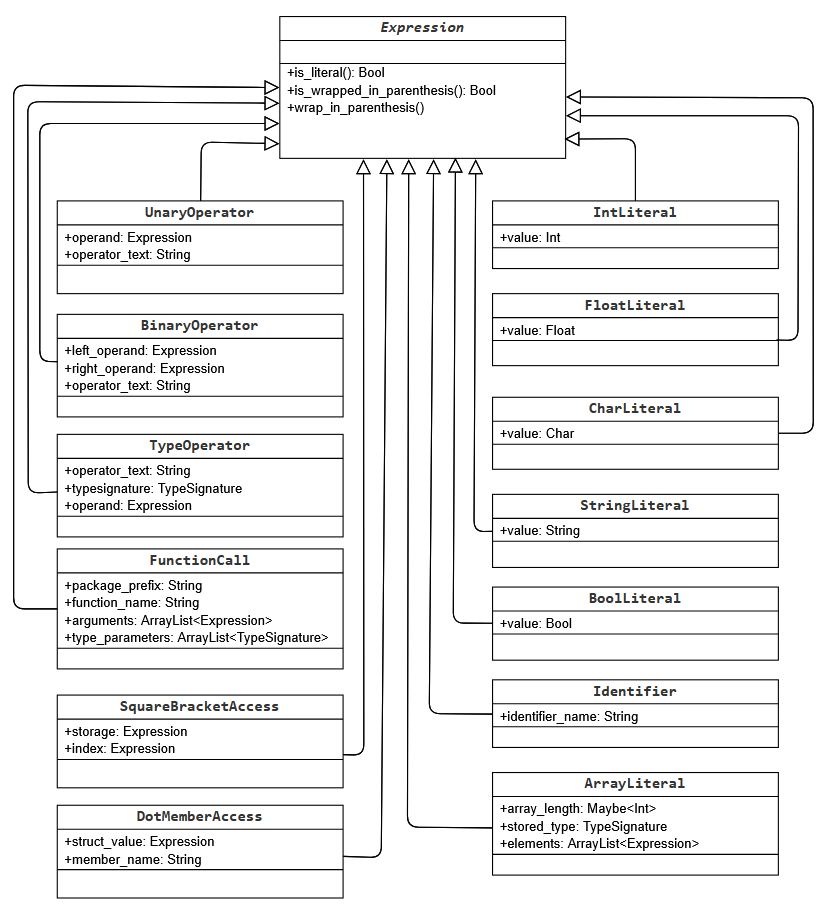
\includegraphics[width=1\textwidth]{../../Assets/AstExpr.png}
    \caption{UML class diagram dei nodi dell'AST che rappresentano espressioni}
\end{figure}

\newpage

Di seguito segue l'UML class diagram relativo alle classi che modellano 
gli statement in forma di AST. Così come già detto, anche la repository
basata su ANTLR utilizza la medesima rappresentazione, e si utilizza il visitor
autogenerato da ANTLR per navigare la rappresentazione di ANTLR e tradurla opportunamente.

\begin{figure}[H]
    \centering
        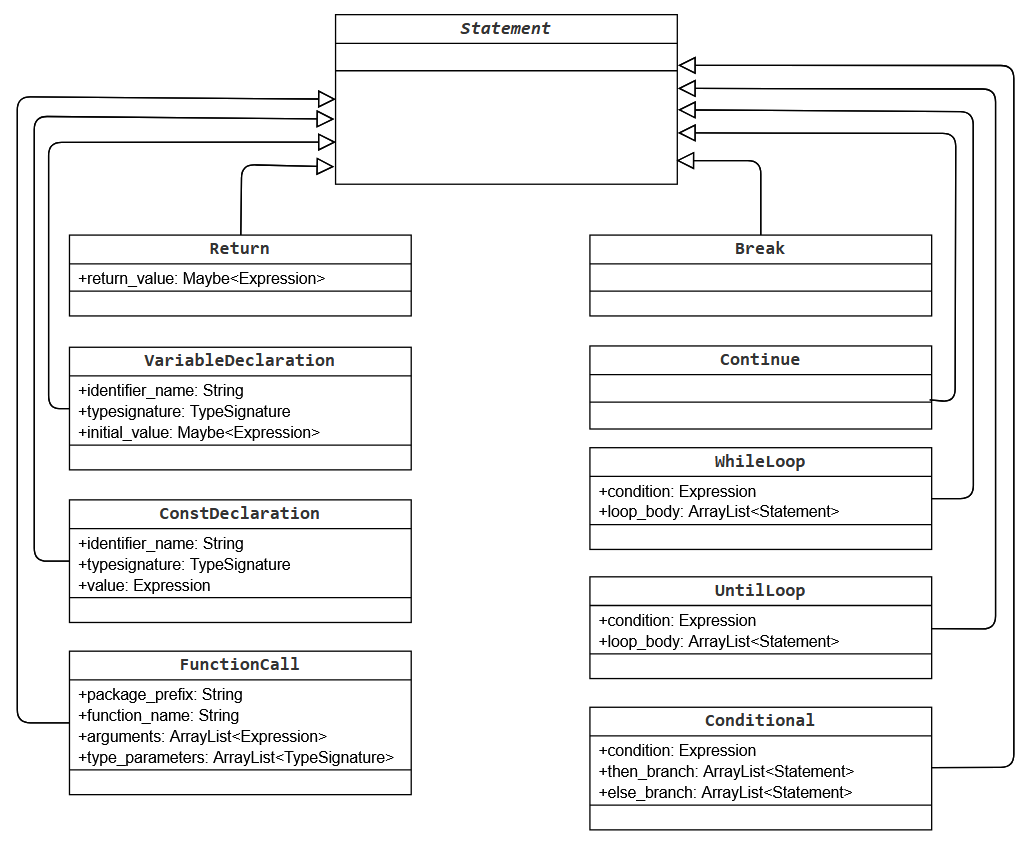
\includegraphics[width=1\textwidth]{../../Assets/StatementAST.png}
    \caption{UML class diagram dei nodi dell'AST che rappresentano statement}
\end{figure}

Si può osservare che la classe \texttt{FunctionCall} è sia un sottotipo di \texttt{Expression}
sia di \texttt{Statement}. Questo è dovuto al fatto che una chiamata di funzione può essere
usata sia come espressione, se restituisce un valore, sia come statement, in caso contrario. \\

Si ricordi infatti che in C++ esiste l'ereditarietà multipla, e quindi è possibile che un
una classe abbia più di un super-tipo anche nei casi in cui si usa l'ereditarietà.

\newpage

Di seguito segue l'UML class diagram relativo alle classi che modellano type-signatures e 
definizioni di tipo in forma di AST. Così come già detto, anche la repository
basata su ANTLR utilizza la medesima rappresentazione, e si utilizza il visitor
autogenerato da ANTLR per navigare la rappresentazione di ANTLR e tradurla opportunamente.

\begin{figure}[H]
    \centering
        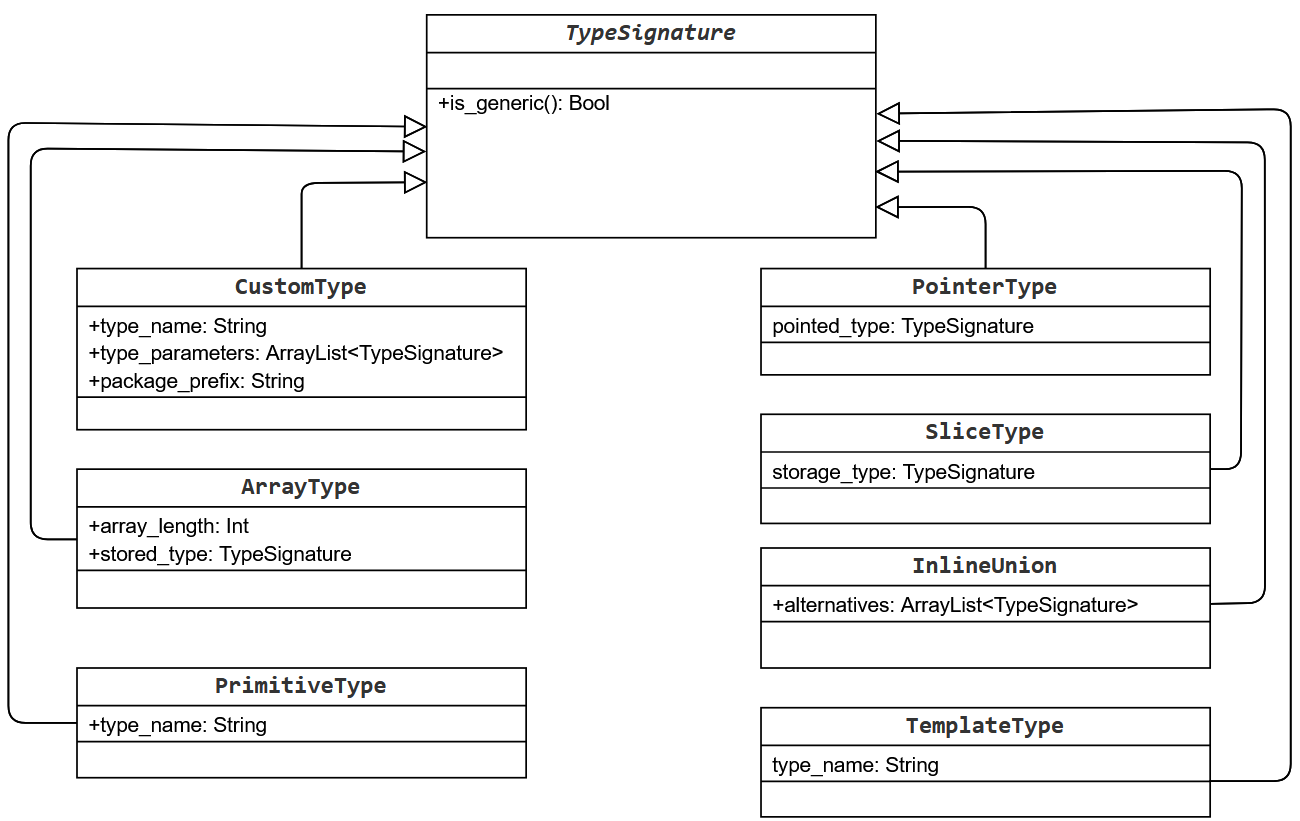
\includegraphics[width=0.9\textwidth]{../../Assets/TypeSignatureAST.png}
    \caption{
        \centering
        UML class diagram dei nodi dell'AST che rappresentano le type-signature
    }
\end{figure}
\vspace{0.5cm}

\subsubsection{Tracciamento delle coordinate}
Ogni classe dell'AST è sotto-tipo propriamente detto (via ereditarietà) della classe \texttt{CoordinatesAwareEntity},
la quale contiene informazioni utilizzabili per fornire messaggi di errore contestualizzati e significativi. \\

Tali informazioni sono dette coordinate, e consentono di tracciare la posizione dell'entità 
(Tipo, Funzione, Statement, Espressione) all'interno del file sorgente. \\

\begin{lstlisting}[language=C++, frame=single]
struct CoordinatesAwareEntity {

    string filename;
    int line_number;
    int tok_number;
    int char_pos;

    /* ... */
};
\end{lstlisting}